\documentclass[11pt]{article}
\usepackage{multicol}
\usepackage{setspace}
\usepackage{graphicx}
\usepackage[margin=1cm,noheadfoot]{geometry} 
\begin{document}
\doublespacing

\begin{center}
\Large \textbf{Formula Reference} \normalsize
\end{center}

\section{General}
\begin{multicols}{2}

\textbf{slope:} $m=\frac{\Delta y}{\Delta x}$ \overrightarrow{} $\Delta y=m\Delta x$ \overrightarrow{} $\Delta x=\frac{\Delta y}{m}$

\textbf{line:} $y=mx+b$, $b=y intercept$

\textbf{circumference:} $c=2\pi r$ \overrightarrow{} $r=\frac{c}{2\pi}$

\textbf{area:} $a=\pi r^2$ \overrightarrow{} $r=\sqrt{\frac{a}{\pi}}$

\textbf{triangle area:} $a=\frac{1}{2}bh$ \overrightarrow{} $h=\frac{2a}{b}$ \overrightarrow{} $b=\frac{2a}{h}$

\textbf{Pythagorus:} $c^2=a^2+b^2$

\textbf{pendulum:} $T=2\pi\sqrt{\frac{L}{g}}$

\end{multicols}

\section{Trigonometry}
\begin{multicols}{2}

$\sin A=\frac{a}{c}$, $\cos A=\frac{b}{c}$

$a=c\sin\theta$, $b=c\cos\theta$

$a^2=b^2+c^2-2b\cos A$, $\frac{\sin C}{c}=\frac{\sin A}{a}$

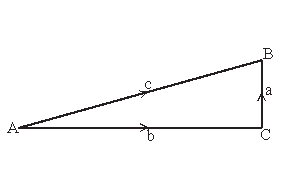
\includegraphics[bb=0 60 0 -50]{triangle.pdf}
\end{multicols}

\section{Motion}
\begin{multicols}{2}

$v=\frac{\Delta d}{\Delta t}$ \overrightarrow{} $d=tv$ \overrightarrow{} $t=\frac{\Delta d}{\Delta v}$

$a=\frac{\Delta v}{\Delta t}$

\textbf{instantaneous} = slope of tangent

\textbf{average} = slope of connecting line

$v_{avg}=\frac{v_{o}+v_{f}}{2}$ \overrightarrow{} $v_{o}=2v_{avg}-v_{f}$ \overrightarrow{} $v_{f}=2v_{avg}-v_{o}$

$a=\frac{v_{f}-v_{o}}{t}$

$d=\frac{1}{2}at^2$ \overrightarrow{} $t=\sqrt{\frac{2d}{a}}$ \overrightarrow{} $a=\frac{2d}{t^2}$

$v_{f}^2=2ad$

$v_{f}=at$

$d=v_{o}t+\frac{1}{2}at^2$

$v_{f}^2=v_{o}^2+2ad$

$v_{f}=v_{o}+at$
\end{multicols}

\section{Forces}
\begin{multicols}{2}

$F=ma$ \overrightarrow{} $a=\frac{F}{m}$ \overrightarrow{} $m=\frac{F}{a}$

$\mu = \frac{F_{f}}{F_{N}}$ \overrightarrow{} $F_{f}=\mu F_{N}$ \overrightarrow{} $F_{N}=\frac{F_{f}}{\mu}$

$weight=mg$ \overrightarrow{} $m=\frac{weight}{g}$ \overrightarrow{} $g={weight}{m}$

$g=9.80\frac{m}{s^2}$ or $\frac{N}{kg}$
\end{multicols}

\section{Gravitation}
\begin{multicols}{2}

$F_{1}r_{1}^2=F_{2}r_{2}^2$

$F=\frac{Gm_{1}m_{2}}{r^2}$

$G=6.67\times 10^-11 \frac{Nm^2}{kg^2}$
\end{multicols}

\section{Momentum}
\begin{multicols}{2}

$p=mv$ \overrightarrow{} $m=\frac{p}{v}$ \overrightarrow{} $v=\frac{p}{m}$

\textbf{Impulse:} $Ft=\Delta (mv)$

$m_{1}v_{1}+m_{2}v_{2}=(m_{1}+m_{2})v_{f}$

$m_{1}v_{1}+m_{2}v_{2}=m_{1}v_{1}^{\prime}+m_{2}v_{2}^{\prime}$

$\frac{1}{2}m_{1}v_{1}^2+\frac{1}{2}m_{2}v_{2}^2=\frac{1}{2}m_{1}v_{1}^{2\prime}+\frac{1}{2}m_{2}v_{2}^{2\prime}$
\end{multicols}

\newpage

\section{Power}
\begin{multicols}{2}

$work=Fd$ \overrightarrow{} $F=\frac{work}{d}$ \overrightarrow{} $d=\frac{work}{F}$

$power=\frac{Fd}{t}$
\end{multicols}

\section{Energy Joules}
\begin{multicols}{2}

$E_{p}=mgh$ \overrightarrow{} $h=\frac{E_{p}}{mg}$ \overrightarrow{} $m=\frac{E_{p}}{gh}$ \overrightarrow{} $g=\frac{E_{p}}{mh}$

$E_{k}=\frac{1}{2}mv^2$ \overrightarrow{} $v=\sqrt{\frac{2E_{k}}{m}}$ \overrightarrow{} $m=\frac{2E_{k}}{v^2}$

$v=\sqrt{2gh}$ \overrightarrow{} $h=\frac{v^2}{2g}$ \overrightarrow{} $g=\frac{v^2}{2h}$
\end{multicols}

\section{Heat}
\begin{multicols}{2}

$\Delta E_{h}=mc(T_{f}-T_{e})$

$C for H_{2}O=4200\frac{J}{kg^{\circ}C}$
\end{multicols}

\section{Waves}
\begin{multicols}{2}

In Hz $f=\frac{1}{T}$ \overrightarrow{} $T=\frac{1}{f}$

$\frac{\sin i}{\sin r}=\frac{v_{x}}{v_{r}}=\frac{\lambda_{x}}{\lambda_{r}}$, $f=constant$

$n_{max}=\frac{d}{\lambda}$

$\sin \theta_{n}=\frac{n_{\theta}}{d}$, anti-nodal lines, sources in phase
\end{multicols}

\section{Light}
\begin{multicols}{2}

$c=299792458\frac{m}{s}$, $\approx 3.00\times 10^8\frac{m}{s}$

\textbf{Snell's Law:} $n=\frac{\sin 1}{\sin r}$, ENTERING dense medium

$n_{1}\sin \theta_{1}=n_{2} \sin \theta_{2}$

$\sin (critical angle)=\frac{n_{1}}{n_{2}}$ $n_{1}$ must be $<n_{2}$

$\frac{h_{i}}{h_{o}}=\frac{d_{i}}{d_{o}}=magnification ratio$

$\frac{h_{o}}{h_{i}}=\frac{d_{o}}{d_{i}}$

\end{multicols}

\singlespacing
\end{document}
